\section{Implementation}
The implementation of the deepfake detection model involves several key stages, from data preprocessing to model evaluation. The overall process can be divided into the following steps:
\begin{figure}[h!]
  \centering
  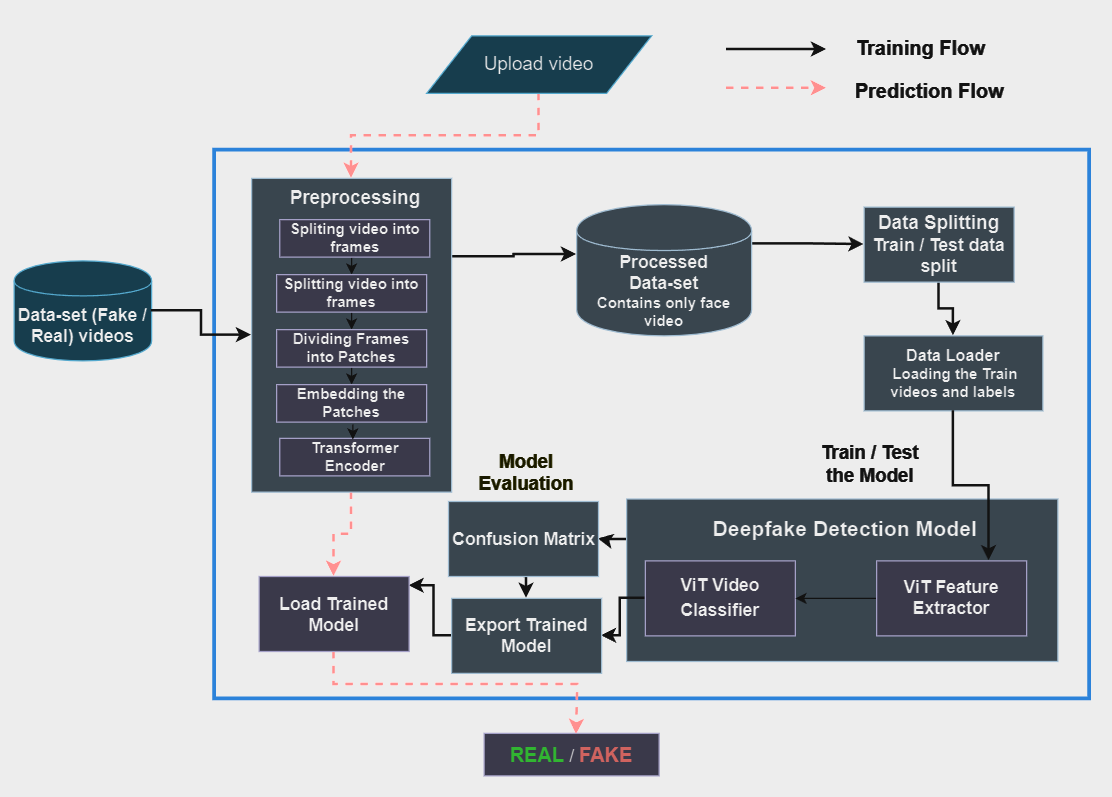
\includegraphics[width=1\textwidth]{images/ViT-App-Architecture.png}
  \caption{Application of Implementation}\cite{df01}
  \label{fig:vit_app_architecture}
\end{figure}
\subsection{Data Preprocessing}
Before training the model, the input videos from the FaceForensics++ dataset undergo preprocessing. The videos are split into individual frames, and face detection is applied to isolate only the facial regions. These cropped facial frames are then resized into consistent dimensions and saved for further use. This step ensures that the model focuses on the facial area, which is critical for detecting subtle manipulations in deepfake videos.
\subsection{Dataset Splitting}
The processed frames are divided into training and testing sets. This splitting allows the model to learn from the training set and generalize to unseen data from the testing set, which helps in evaluating its performance.
\subsection{Loading Data with DataLoader}
A DataLoader is utilized to efficiently load batches of data (videos and their corresponding labels) into the model during training. This process ensures that the GPU/CPU is optimally used by feeding data in manageable chunks, reducing memory overhead, and speeding up the training process.
\subsection{Model Training}: The model is trained using a supervised learning approach, with the video labels (real or fake) serving as the ground truth. The training process involves optimizing the model's parameters using a loss function (e.g., cross-entropy loss) and an optimizer like Adam. During training, the model learns to minimize the error between its predictions and the actual labels by updating its internal weights.
\subsection{Evaluation and Testing}
After training, the model is evaluated on the test set using metrics such as accuracy, precision, recall, and F1-score. A confusion matrix is generated to assess the model’s performance in distinguishing between real and fake videos. The trained model is then exported for deployment.